% Chapter Template

\chapter{Глибинне навчання} % Main chapter title

\label{Chapter4} % Change X to a consecutive number; for referencing this chapter elsewhere, use \ref{ChapterX}

Як зазначено у попередньому роздiлi (Роздiл \ref{Chapter3}), фрактальний аналiз текстури iнтерфаз- ного ядра букального епiтелiю i взагалi будь-який алгоритм класифiкацiї, який викорис- товує характеристики текстури та контуру ядра клiтини, добре розпiзнають клас здоро- вих пацiєнтiв вiд пацiєнтiв, хворих раком молочної залози чи фiброаденоматозом, але майже не можуть роздiляти останнi два класи мiж собою. Це пояснюється тим, що цi хвороби викликають дуже схожi гормональнi реакцiї, що призводить до схожих змiн у ядрах ДНК клiтин букального епiтелiю.

Цей роздiл буде присвячено задачi класифiкацiї тiльки класiв хворих раком та фiбро- аденоматозом. За допомогою технiк глибинного машинного навчання, ми намагаємося аналiзувати та використовувати локальнi ознаки та особливостi текстури поверхнi ядра клiтини, якi не можна характеризувати одним числом. 

%----------------------------------------------------------------------------------------
%	SECTION 1
%----------------------------------------------------------------------------------------

\section{Нейронні мережі}

\begin{figure}[b!]
	\minipage{0.5\textwidth}
	\centering	
	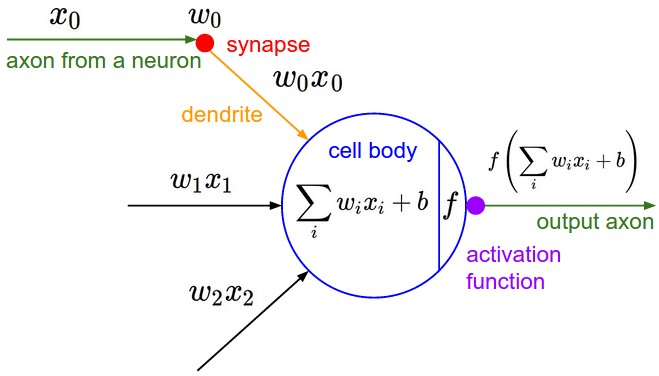
\includegraphics[width=0.90\linewidth]{Figures/Chapter4/neuron_model.jpeg}\\
	(a)
	\endminipage\hfill
	\minipage{0.5\textwidth}
	\centering	
	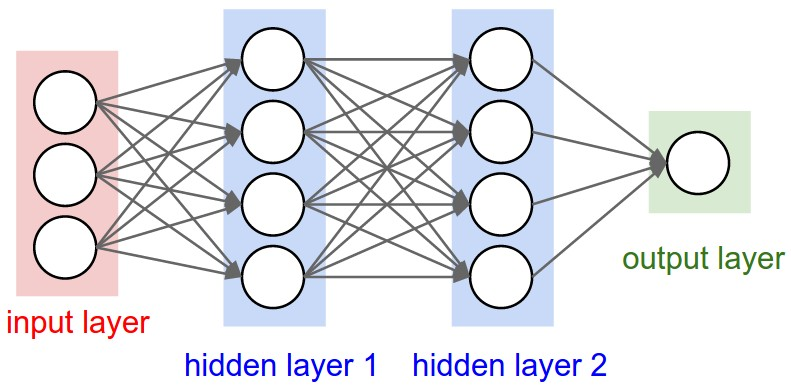
\includegraphics[width=0.90\linewidth]{Figures/Chapter4/neural_net2.jpeg}\\
	(б)
	\endminipage\hfill
	
	\caption{Структура одного нейрону (а) та схема багатошарових перцептронів як граф потоку сигналів (б).}
	\label{fig:neuralnet}
\end{figure}

Штучна нейронна мережа -- це математична модель, яка побудована за принципом функ- цiонування бiологiчних нейронних мереж. Штучнi нейроннi мережi широко використо- вують для задач машинного навчання, розпiзнавання образiв, дискримiнантного аналiзу, кластерування тощо. 

Нейронну мережу можна iнтерпретувати як граф. У підручнику \citep{book:haykin}, нейроннi мережi описуються як граф потоку сигналу (signal-flow graph), де кожен нейрон (або вершина у графi) є окремою одиницею обчислення. Схема одного штучного нейрону зображена на (Мал. \ref{fig:neuralnet} (а)).

Кожен нейрон мережi має справу лише з сигналами, якi вiн перiодично отримує, i сигналами, якi вiн перiодично надсилає iншим нейронам. i тим не менш, будучи з'єдна- ними в достатньо велику мережу з керованою взаємодiєю, такi простi нейрони разом здатнi моделювати складнi функцiї, виявляти складнi залежностi мiж вхiдними й вихiд- ними даними, а також здiйснювати узагальнення.


\subsection{Багатошаровий перцептрон}

Штучний багатошаровий перцептрон -- це така архiтектура нейронних мереж, у якiй групи нейронiв формують \enquote{шари}, в яких кожний нейрон з одного шару зв'язана з усiма нейронами сусiднього шару. Отже, сигнали на вихiд одного шару нейронiв є сигналами на вхiд нейронiв наступного шару. На (Мал. \ref{fig:neuralnet} (б)) зображено схему багатошарового перцептрону. Такi шари нейронiв також називають \enquote{повнiстю зв'язаними} (Fully connected layers).

\subsection{Функція активації ReLU}

У цiй роботi було використано функцiю зрiзаних лiнiйних вузлiв, або ReLU, для активацiї нейронiв замiсть сигмоїдальних функцiй чи гiперболiчного тангенсу. Функцiя активацiї ReLU (Rectified Linear Unit), яка задається наступним чином:

\begin{equation*}
f(x) = \max(0, x)
\end{equation*}

має багато переваг над сигмоїдальними функцiями чи гiперболiчним тангенсом при використаннi в якостi функцiї активацiї:

\begin{itemize}
	\item В роботi \parencite{nn:krizhevsky_imagenet}, було доведено що така функцiя активацiї може прискорити збiжнiсть спуску за градiєнтом до 6 разiв у порiвняннi з сигмоїдальними функцiями чи гiперболiчними тангенсами.
	
	\item Сигмоїдальнi функцiї та гiперболiчнi тангенси використовують складнi операцiї, такi як зведення у степiнь.
\end{itemize}

Детальний аналiз переваг та недолiкiв цiєї функцiї, а також позбавлення недолiкiв за допомогою модифiкованої версiї \enquote{Leaky ReLU}, описаний в роботi \parencite{nn:kaiming}.


\subsection{Згорткові нейронні мережі}

Згортковi нейроннi мережi -- це мережi, якi мiстять згортковi шари нейронiв, уперше запропонований \parencite{nn:lecun_cnn}. Згортковий шар нейронiв мiстить фiльтри -- набiр ваг. При подачi даних на вхiд, вихiдний сигнал обчислюється як згортка фiльтру з локальним регiоном зображення. На (Мал. \ref{fig:convonet} (а)) показано схему першого згорткового шару, де кожен нейрон локально зв'язаний з пiкселями зображення та \enquote{бачить} усi канали. Кiлькiсть шарiв нейронiв у згортковому шару (зображено кружечками) дорiвнює кiлькостi фiльтрiв згорткового шару, тобто для рiзних шарiв нейронiв використовується рiзнi фiльтри.

Згортковi нейроннi шари використовують для виявлення локальних особливостей зобра- ження. Цi шари також дозволяють мережi бути бiльш стiйкою до трансляцiї, тобто надають деяку iнварiантнiсть. Тому, будемо використовувати згортковi шари для побу- дови класифiкатора мiж хворими раком та фiброаденоматозом.

Разом iз згортковими нейронними шарами також будемо використовувати пiдвибiрковi шари (pooling layers), якi значно зменшують обсяг вхiдних даних на наступнi шари мережi.

\begin{figure}[t!]
	\minipage{0.4\textwidth}
	\centering	
	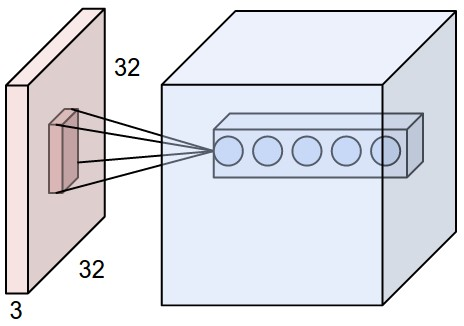
\includegraphics[width=0.90\linewidth]{Figures/Chapter4/depthcol.jpeg}\\
	(a)
	\endminipage\hfill
	\minipage{0.6\textwidth}
	\centering	
	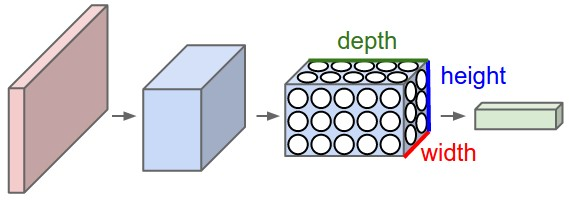
\includegraphics[width=0.90\linewidth]{Figures/Chapter4/cnn.jpeg}\\
	(б)
	\endminipage\hfill
	
	\caption{На (а) схематично зображено згортковий шар. На (б) зображено схему згорткової мережі.}
	\label{fig:convonet}
\end{figure}

\subsection{Алгоритм RMSProp}

Пiсля обчислення градiєнтiв за допомогою алгоритму зворотного поширення помилок (backpropagation), цi градiєнти використовуються для оновлення параметрiв (ваг) ней- ронної мережi. Зазначимо, що оптимiзацiя алгоритму оновлення нейронних мереж є на момент написання цiєї роботи дуже активною сферою дослiджень.

Алгоритм RMSProp \citep{nn:rmsprop} є дуже ефективним, але ще не опублiкований метод адаптивного оновлювання параметрiв. Вiн налаштовує та регулює алгоритм Adagrad \parencite{nn:adagrad} таким чином щоб зменшити рiзкiсть монотонного зменшення швидкостi навчання. На вiдмiну вiд Adagrad, цей алгоритм використовує так званi \enquote{ковзаючi} середньоквадратичнi значення градiєнтiв:

\begin{equation*}
cache = decay\_rate \cdot cache + (1 - decay\_rate) \cdot dx^2
\end{equation*}
\begin{equation*}
x = x - \frac{learning\_rate \cdot dx}{\sqrt{cache} + eps}
\end{equation*}

де \(decay\_rate\) це гiперпараметр, якому зазвичай присвоюють значення з множини чисел \(\{0.9, 0.99, 0.999\}\). Отже, метод RMSProp також модулює швидкiсть навчання кожного параметру з урахуванням величин його градiєнтiв, що має вигiдний ефект вирiвнювання. Але, на вiдмiну вiд Adagrad, величини оновлень не зменшуються монотонно.

У цiй роботi використовується саме алгоритм RMSProp. На практицi бiльш стандартним методом для оновлення параметрiв є алгоритм Adam (adaptive moment estimation) \parencite{nn:adam}, який дуже схожий на RMSProp та у деяких випадках є трохи ефективнiшим нiж RMSProp, але цей алгоритм є бiльш громiздким та потребує трохи бiльше часу для обчислень. Повний алгоритм Adam також включає механiзм корекцiї змiщень. Альтернативою RMSProp та Adam є також комбiнацiя алгоритмiв SGD та Nesterov Momentum.

\subsection{Регуляризація нейронної мережі}

\begin{figure}[t]
	\centering
	\minipage{0.7\textwidth}
	\minipage{0.5\textwidth}
	\centering	
	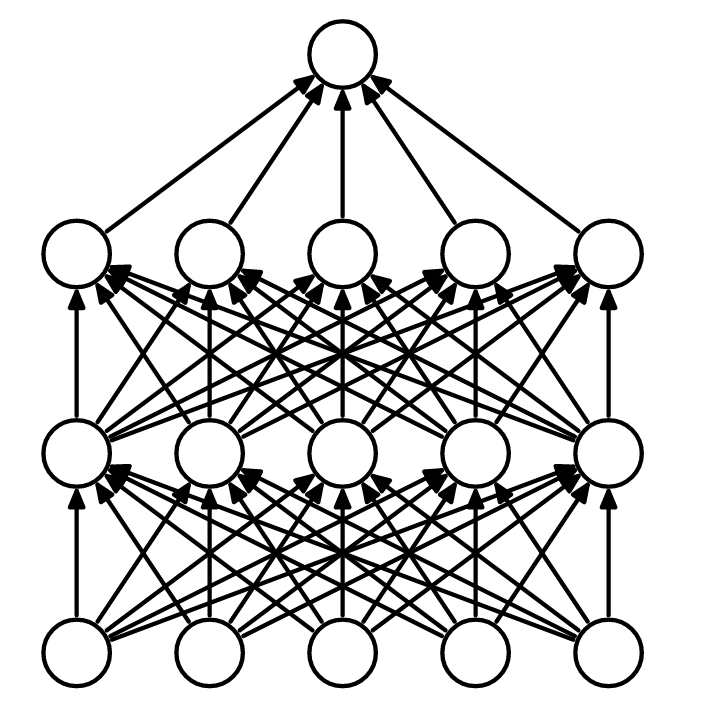
\includegraphics[width=0.8\linewidth]{Figures/Chapter4/dropout1.png}
	\\ (а) До Dropout
	\endminipage\hfill
	\minipage{0.5\textwidth}
	\centering	
	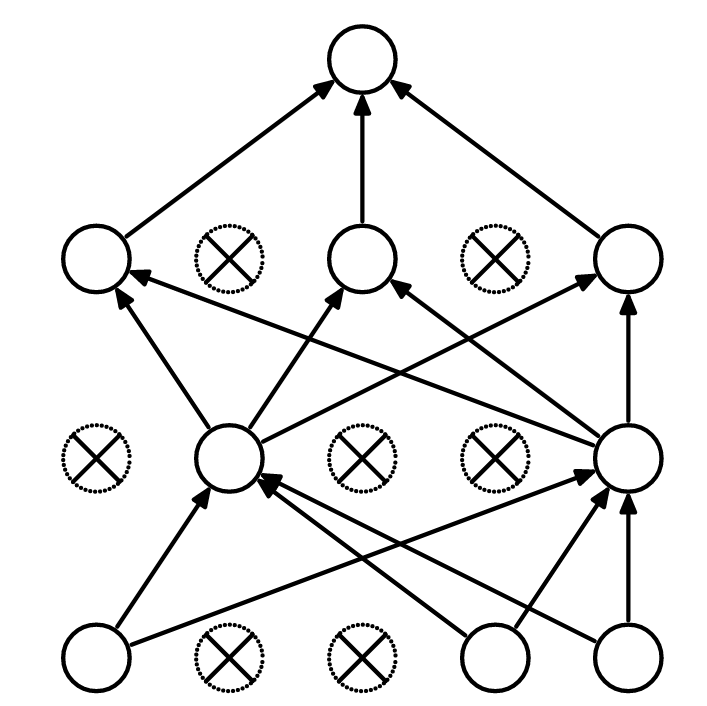
\includegraphics[width=0.8\linewidth]{Figures/Chapter4/dropout2.png}
	\\ (б) Після Dropout
	\endminipage\hfill
	\endminipage\hfill
	
	\caption{Візуалізація методу Dropout з ймовірністю \(p = 0.5\).}
	\label{fig:dropout}
\end{figure}

Процес регуляризацiї нейронної мережi -- це процес уникнення перенавчання (overfitting) мережi. iснує кiлька способiв контролювання тренування нейронної мережi, щоб максимальним чином уникнути перенавчання.

У цiй роботi використовується метод Dropout -- простий та дуже ефективний метод регуляризацiї, запропонований \parencite{nn:dropout}. При тренуваннi, кожен нейрон є активним за ймовiр- нiстю \(p\) (що є гiперпараметром мережi).

На (Мал. \ref{fig:dropout}) схематично зображено принцип роботи методу Dropout. На практицi також часто використовують алгоритми \(L1\)- та \(L2\)- регуляризацiї нейронних мереж \citep{nn:l1l2regularization}, разом з методом Dropout.

\subsection{Функція втрат. Перехрестна ентропія.}

Вибiр функцiї втрат є одним з найважливiших крокiв при побудовi моделi класифiкатора. Вдало обрана функцiя втрат може значно покращити результат та швидкiсть тренування класифiкатора.

На практицi при тренуваннi класифiкаторiв на основi нейронних мереж найчастiше використовують перехресну ентропiю (categorical crossentropy):
\begin{equation*}
L_i = -\log\left(\frac{e^{f_{y_i}}}{ \sum_j e^{f_j} }\right)
\end{equation*}

яка для випадку задач класифiкацiї дає кращi результати, нiж середньоквадратична функцiя втрат (mean square error) та функцiя помилки класифiкацiї (classification error). У цiй роботi використовується саме ця функцiя оцiнювання втрат. Слiд також зазначити, що при тренуваннi моделi та при класифiкацiї чи обчисленнi можна використовувати рiзнi оцiнки втрат.

%----------------------------------------------------------------------------------------
%	SECTION 2
%----------------------------------------------------------------------------------------

\section{Класифікація за допомогою нейронних мереж}


\subsection{Прирощення даних}

Як вказано у роздiлi \ref{Chapter1}, для дослiдження маємо тiльки набiр даних який мiстить 3403 зображень iнтерфазних ядер букального епiтелiю, взятих з 68 пацiєнтiв хворих раком молочної залози, та 1741 зображень ядер взятих з 33 пацiєнтiв хворих фiброаденоматозом. Така кiлькiсть є дуже малою для тренування глибоких згорткових нейронних мереж. Отже, будемо штучно збiльшувати кiлькiсть даних для тренування.  

При подачi в нейронну мережу випадковим чином зробимо декiлька з наступних пере- творень над зображеннями:
\begin{itemize}
\item Перевернути зображення вiдносно горизонтальної осi
\item Перевернути зображення вiдносно вертикальної осi
\item Повернути зображення на випадковий кут вiд \(0\) до \(2\pi\), при чому пiкселi, що до перетворення знаходилися за межами входу, присвоюються значенню сусiднiх пiк- селiв.
\end{itemize}

\begin{figure}[t!]
	\minipage{0.2\textwidth}
	\centering
	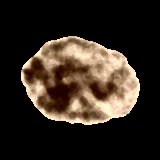
\includegraphics[width=0.97\linewidth]{Figures/Chapter4/aug_0.png}	
	\endminipage\hfill
	\minipage{0.2\textwidth}
	\centering	
	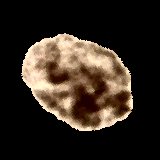
\includegraphics[width=0.97\linewidth]{Figures/Chapter4/aug_1.png}
	\endminipage\hfill
	\minipage{0.2\textwidth}
	\centering	
	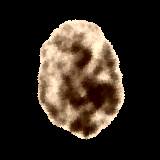
\includegraphics[width=0.97\linewidth]{Figures/Chapter4/aug_2.png}
	\endminipage\hfill
	\minipage{0.2\textwidth}
	\centering	
	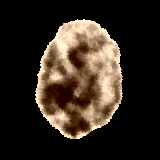
\includegraphics[width=0.97\linewidth]{Figures/Chapter4/aug_3.png}
	\endminipage\hfill
	\minipage{0.2\textwidth}
	\centering	
	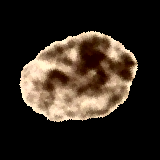
\includegraphics[width=0.97\linewidth]{Figures/Chapter4/aug_4.png}
	\endminipage\hfill	
	
	\caption{Прирощення даних на прикладі одного зображення.}
	\label{fig:data_augmentation}
\end{figure}


\subsection{Проблема незбалансованості вибiрки для тренування}

Для тренування було обрано випадковим чином \(80\%\) вiд всього набору даних. Це стано- вить 1392 зображень взятих з 33 пацiєнтiв хворих фiброаденоматозом та 2722 зображень з 68 пацiєнтiв хворих раком молочної залози. Отже, в набiр даних для валiдацiї входять iншi зображення ядер букального епiтелiю тих самих пацiєнтiв. Маємо незбалансованiсть вибiрки для тренування, де кiлькiсть даних з одного класу (з класу хворих раком) майже вдвiчi перевищує кiлькiсть даних з iншого класу (хворих фiброаденоматозом). 

Незбалансованiсть набору даних для тренування може значно негативно вплинути на навчання класифiкатора \citep{nn:imbalance2}. Слiд зазначити, що набiр даних для валiдацiї теж є незба- лансованим. Так, пiсля тренування моделi на незбалансованiй вибiрцi, автором цiєї робо- ти було отримано класифiкатор, точнiсть розпiзнавання якого на обох наборах даних для тренування i тестування становила бiльш нiж 65\%. Подальший аналiз результатiв виявив, що отримана модель має чутливiсть, близьку до 100\% та специфiчнiсть, близьку до 0\%, тобто модель у бiльшостi випадкiв просто класифiкувала зображення як \enquote{нале- жить хворого раком}. Отже, необхiдно знайти спосiб боротьби з проблемою незбалансо- ваностi набору даних для тренування.

Існує багато методiв для боротьби з цiєю проблемою. Найбiльш поширеними на практицi є методи змiни об'єму даних (subsampling methods) та методи навчання з вагами (cost-sensitive methods) \citep{nn:imbalance}, де рiзним класам присвоюється деяке значення \enquote{критичностi} помилки. Було вирiшено використовувати перший метод.

Отже, пiсля змiни об'єму даних, кiлькiсть зображень для тренування становить 1392 з хворих фiброаденоматозом та 1632 з хворих раком молочної залози, а кiлькiсть зобра- жень для валiдацiї становить 349 зображень з хворих фiброаденоматозом та 1771 зобра- жень з хворих раком молочної залози.

\subsection{Архітектура мережі}

Для зручного опису архiтектури мереж, використаємо наступнi позначення:

\begin{itemize}
	\item Позначимо повністю зв'язані шари нейронів (fully-connected layers) як \(xFC\), де \(x\) -- кількість нейронів шару. Наприклад, якщо повністю зв'язаний шар має 128 нейронів, то позначаємо \(128FC\).
	
	\item Згорткові нейронні шари (convolutional layers), де фільтри шару мають розміри \(x \times x\), позначимо як \(yCONVx\), де \(y\) -- кількість фільтрів. Наприклад, \(64CONV3\).
	
	\item Підвибіркові шари (max-pooling layers) позначимо як \(MPx\), де \(x\) -- розмір ядра фільтру. Наприклад, \(MP2\).
	
	\item Вхідні (input) та вихідні (output) дані позначимо як \(I\) та \(O\) відповідно.
	
	\item Домовимось, що сигнал протікає з шару, що знаходиться лівіше у записі, до шару, що знаходиться правіше. Сусідні шари нейронів з'єднуємо символом \enquote{\(\rightarrow\)}. Повна архітектура мережі так: \(I \rightarrow 32CONV3 \rightarrow MP2 \rightarrow FC16 \rightarrow O\).
\end{itemize}

Автором було розглянуто багато рiзних архiтектур нейронної мережi. Окрiм простих вiдносно неглибоких архiтектур згорткової нейронної мережi, якi схожi на AlexNet, також були розглянутi мережi, подiбнi до VGG \cite{nn:vgg}.

\bigskip
\begin{itemize}
	\label{arch}
	
	\item[ARCH-0]
	\(I \rightarrow
	32CONV3 \rightarrow
	MP2 \rightarrow
	32CONV3 \rightarrow
	MP2 \rightarrow
	64CONV5 \rightarrow
	MP2 \rightarrow
	FC32 \rightarrow
	FC32 \rightarrow
	O \)
	
	\item[ARCH-1]
	\(I \rightarrow
	32CONV3 \rightarrow
	MP2 \rightarrow
	48CONV3 \rightarrow
	MP2 \rightarrow
	64CONV3 \rightarrow
	MP2 \rightarrow
	72CONV3 \\ \rightarrow 
	MP2 \rightarrow
	FC64 \rightarrow
	FC64 \rightarrow
	O \)
	
	\item[ARCH-2]
	\(I \rightarrow
	64CONV5 \rightarrow
	48CONV3 \rightarrow
	MP2 \rightarrow
	FC32 \rightarrow
	FC16 \rightarrow
	O \)
	
	\item[ARCH-3]
	\(I \rightarrow
	64CONV3 \rightarrow
	MP2 \rightarrow
	64CONV3 \rightarrow
	MP2 \rightarrow
	96CONV3 \rightarrow
	MP2 \rightarrow
	96CONV3 \\ \rightarrow
	MP2 \rightarrow
	FC48 \rightarrow
	FC48 \rightarrow
	O \)
		
	\item[VGG-9]
	\(I \rightarrow
	32CONV3 \rightarrow
	32CONV3 \rightarrow
	MP2 \rightarrow
	48CONV3 \rightarrow
	48CONV3 \rightarrow
	MP2 \rightarrow
	64CONV5 \rightarrow
	64CONV5 \rightarrow
	MP2 \rightarrow
	FC32 \rightarrow
	FC32 \rightarrow
	O \)
	
	\item[VGG-11]
	\(I \rightarrow 
	48CONV3 \rightarrow 
	48CONV3 \rightarrow 
	MP2 \rightarrow 
	64CONV3 \rightarrow 
	64CONV3 \rightarrow 
	MP2 \rightarrow 
	72CONV3 \rightarrow 
	72CONV3 \rightarrow 
	MP2 \rightarrow 
	96CONV3 \rightarrow 
	96CONV3 \rightarrow 
	MP2 \rightarrow
	FC96 \rightarrow
	FC96 \rightarrow
	O \)
	
	\item[VGG-13]
	\(I \rightarrow 
	32CONV3 \rightarrow 
	32CONV3 \rightarrow 
	MP2 \rightarrow 
	64CONV3 \rightarrow 
	64CONV3 \rightarrow 
	MP2 \rightarrow 
	128CONV3 \rightarrow 
	128CONV3 \rightarrow 
	MP2 \rightarrow 
	256CONV3 \rightarrow 
	256CONV3 \rightarrow 
	MP2 \rightarrow
	256CONV3 \rightarrow 
	256CONV3 \rightarrow 
	MP2 \rightarrow
	FC128 \rightarrow
	FC128 \rightarrow
	O \)
\end{itemize}

Для кожного шару нейронiв цих архiтектур було використано ReLU в якостi функцiї активацiї, а для кiнцевого шару \(O\) з одного нейрону (якщо на виходi 0 то зображення класифiкується як належним до хворого раком молочної залози, а якщо 1 -- то класифi- кується як належним до хворого фiброаденоматозом) було використано функцiю актива- цiї SoftMax. З метою регулювання, для кожного повнiстю зв'язаного шару було викорис- тано алгоритм Dropout. В якостi алгоритму задання швидкостi навчання (тобто оновлення параметрiв) використовується RMSProp.


\subsection{Тренування мереж та результати}

\begin{figure}[t!]
	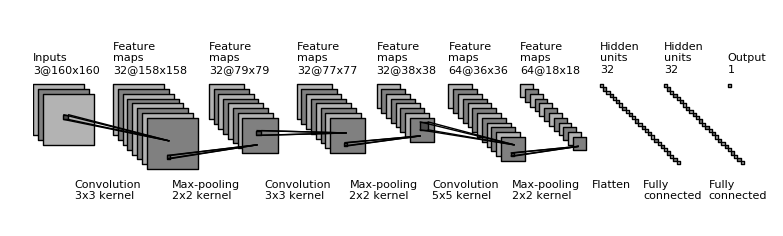
\includegraphics[width=\linewidth]{Figures/Chapter4/best_model.png}
	\caption{Архітектура найкращої мережі.}
	\label{fig:best_model}
\end{figure}

Слiд зазначити, що вибiр архiтектури обмежувався потужнiстю доступних автору обчис- лювальних ресурсiв. У розпорядженнi автора на момент дослiдження був комп'ютер з процесором Intel Core i7, комп'ютер з процесором Intel Core i3, а також вiдеокарта Nvidia Geforce GT 520M. Отже, використання бiльш глибоких нейронних мереж, або мереж з бiльшою кiлькiстю вiльних параметрiв, не було можливим.

Кожна з перерахованих вище мереж тренувалася по декiлька (для ARCH-0 -- декiлька десяткiв) разiв, кожен раз нейронна мережа iнiцiалiзувалася випадковим набором ваг (параметрiв) та навчалася протягом 300 епох. Кожна епоха -- це цикл, в якому нейронна мережа навчається на даних, якi по обсягу дорiвнюють об'єму тренувальної вибiрки. Неповторнiсть вхiдних даних для тренування гарантує алгоритм прирощення даних. Також були використанi рiзнi значення для Dropout, вiд \(0.2\) до \(0.5\).

Сумарно навчання вищеописаних мереж проводилось протягом трьох тижнiв. Найбiльш повiльними для навчання є моделi VGG-9, VGG-11 та VGG-13. У середньому на навчання цих моделей протягом 300 епох пiшло бiльш нiж 48 годин процесорного часу.

Найбiльш вдалою є архiтектура ARCH-0, яка схематично зображена на (Мал. \ref{fig:best_model}). Нижче у таблицi приведенi найкращi результати класифiкацiї окремого зображення iнтерфаз- ного ядра клiтини букального епiтелiю цих мереж.

\bigskip
\begin{center}
\begin{tabular}
{| m{3cm} || m{3cm} | m{3cm} | m{3cm} |}
\hline
Архітектура & Чутливість & Специфічність & Точність \\ \hline \hline
ARCH-0 & 59.17\%  & 67.33\%  & 62.93\%  \\ \hline
ARCH-1 & 55.74\%  & 57.59\%  & 56.60\%  \\ \hline
ARCH-2 & 67.24\%  & 53.58\%  & 60.95\%  \\ \hline
ARCH-3 & 56.72\%  & 58.45\%  & 57.52\%  \\ \hline
VGG-9  & 55.25\%  & 59.89\%  & 57.39\%  \\ \hline
VGG-11 & 58.43\%  & 58.45\%  & 58.44\%  \\ \hline
VGG-13 & 56.23\%  & 55.59\%  & 55.94\%  \\ \hline
\end{tabular}
\end{center}
\bigskip

Найкращi результати за точнiстю дає мережа ARCH-0. Надалi будемо детальнiше аналi- зувати її результати та намагатися побудувати класифiкатор з кращими результатами на основi цiєї моделi.

Можна розглядати кожне зображення ядра клітини певного пацієнта не окремо, а у сукупності з іншими зображеннями клітин цього пацієнта, тобто класифікувати не належ- ність окремого ядра букального епітелію до класу хвороби, а належність самого пацієнта до цих класів. Наприклад, якщо більшість зображень ядер клітин цього пацієнта класи- фікується належними до класу \enquote{хворі раком}, то віднесемо цього пацієнта до класу \enquote{хворий раком} (аналогічно з фіброаденоматозом). Тоді отримаємо наступні результати:


\begin{center}
	\begin{tabular}
		{| m{3cm} || m{3cm} | m{3cm} | m{3cm} |}
		\hline
		Архітектура & Чутливість & Специфічність & Точність \\ \hline \hline
		ARCH-0 & 58.82\%  & 69.70\%  & 62.38\%  \\ \hline
	\end{tabular}
\end{center}

що незначно вiдрiзняються вiд результатiв, отриманих при класифiкацiї окремих клiтин.

\subsection{Аналіз результатів}

Помiтимо, що мережа з вiдносно простою архiтектурою ARCH-0 дає кращi результати нiж VGG-подiбнi мережi. Це можна пояснити тим, що VGG-подiбнi глибокi архiтектури мiстять у декiлька десяткiв разiв бiльше вiльних параметрiв, а отже, потребують бiльше нiж 300 епох для навчання. При тренуваннi моделi VGG-11, наприклад, спостерiгалося дуже вiльне спадання значення функцiї втрат. Це свiдчить про те, що, можливо, треба було обирати iншi гiперпараметри для мережi, такi як \(learning\_ rate\) для алгоритму RMSProp, або використовувати менший \(batch\_size\) (обсяг даних при тренуваннi, пiсля якого обчислюється градiєнт та виконується одне оновлення параметрiв).

\section{Підвищення якості розпізнавання}

Надалi будемо будувати бiльш точний класифiкатор на основi отриманої моделi нейрон- ної мережi ARCH-0. Щоб переконатися у тому, що ця модель дiйсно генералiзується на невiдомi данi (тi, якi не було використано при тренуваннi), розглянемо розподiл вихiдних значень мережi для обох наборiв: тренування та валiдацiї, що показанi на (Мал. \ref{fig:train_distribution}). Можна побачити, що отримана мережа добре генералiзується на вибiрцi для валiдацiї.

\begin{figure}[t!]
	\minipage{0.5\textwidth}
	\centering	
	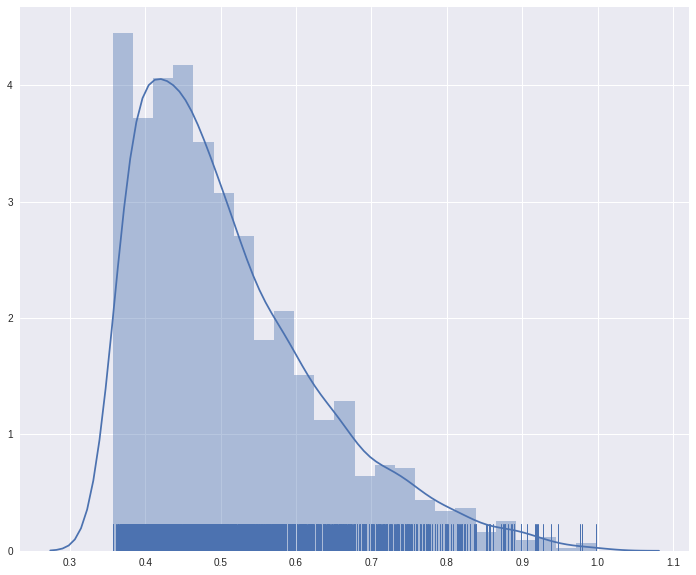
\includegraphics[width=0.95\linewidth]{Figures/Chapter4/train_dist_cancer.png}\\
	(a)
	\endminipage\hfill
	\minipage{0.5\textwidth}
	\centering	
	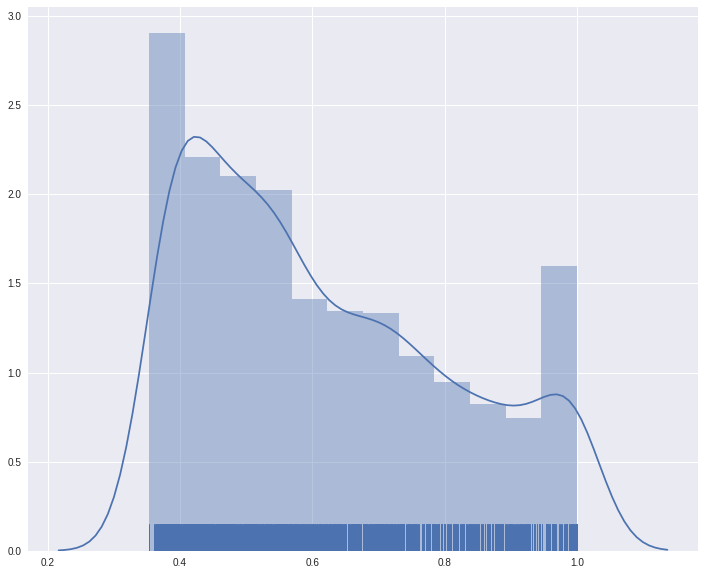
\includegraphics[width=0.95\linewidth]{Figures/Chapter4/train_dist_fibro.png}\\
	(б)
	\endminipage\hfill
	\\	
	\minipage{0.5\textwidth}
	\centering	
	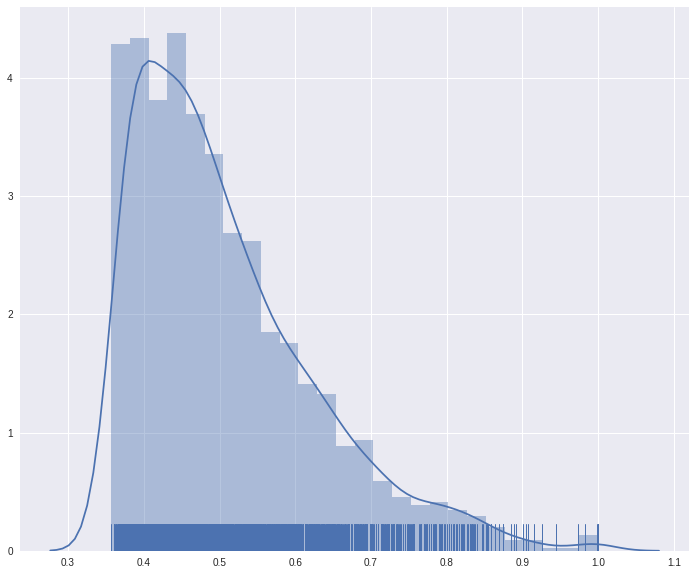
\includegraphics[width=0.95\linewidth]{Figures/Chapter4/test_dist_cancer.png}\\
	(в)
	\endminipage\hfill
	\minipage{0.5\textwidth}
	\centering	
	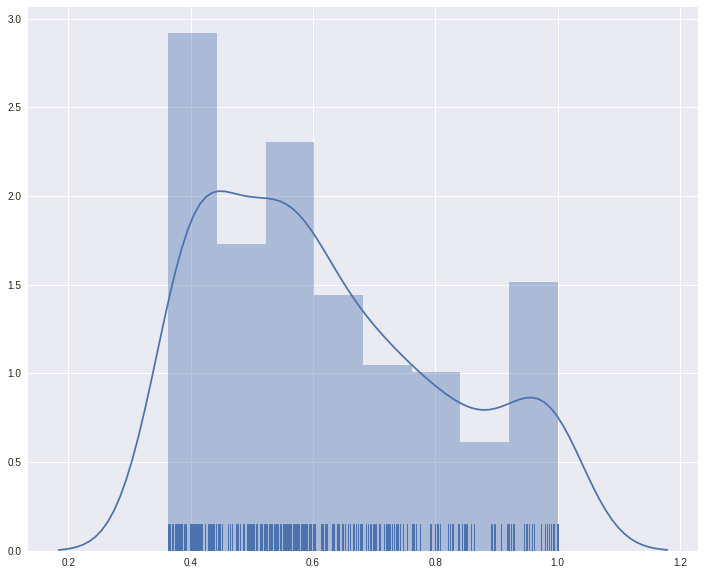
\includegraphics[width=0.95\linewidth]{Figures/Chapter4/test_dist_fibro.png}\\
	(г)
	\endminipage\hfill
	
	\caption{Розподіл значення виходу мережі на зображеннях ядер с вибірки для тренування, що належить пацієнтам хворі на рак (а) та на фіброаденоматоз (б). На (в) та (г) зображено розподіл виходу мережі на зображеннях ядер з вибірки для тестування що належить пацієнтам хворі на рак та фіброаденоматоз відповідно.}
	\label{fig:train_distribution}
\end{figure}

Отже, припускаючи, що розподiл вихiдних значень мережi для пацiєнтiв з однаковою хворобою (рак молочної залози чи фiброаденоматоз) буде також приблизно однаковими, замiсть простого пiдходу, що описаний у попередньому пiдроздiлi, можна розглядати нейронну мережу не як бiнарний класифiкатор, а як генератор ознак, тобто кожному зображенню ставити у вiдповiднiсть деяке число (ознаку). Отже, до кожного пацiєнта (набору зображень) можна застосовувати статистичнi тести.



\subsection{Гибрідний класифікатор}

В якостi критерiю еквiвалентностi генеральних сукупностей було використано критерiй Колмогорова-Смiрнова, що є одним з найефективнiших непараметричних критерiїв для порiвняння вибiрок. Альтернативно можна використовувати \(p\)-статистику, що детально описана у попередньому роздiлi. 

Нехай \(can\_trainX\) -- сукупнiсть зображень iнтерфазних ядер букального епiтелiю у вибiрцi для тренування, взятих з пацiєнтiв хворих раком, а \(fib\_trainX\) -- сукупнiсть зображень ядер у вибiрцi для тренування взятих з пацiєнтiв хворих фiброаденоматозом.  

При класифiкацiї деякого пацiєнта \(P = \{X^1, X^2, \dots X_n\} \) обчислюється: 
\begin{equation*}
can\_train = \textup{ARCH-0}(can\_trainX) = \{\textup{ARCH-0}(X)\,\, \forall X \in can\_trainX\}
\end{equation*}
\begin{equation*}
fib\_train = \textup{ARCH-0}(fib\_trainX) = \{\textup{ARCH-0}(X)\,\, \forall X \in fib\_trainX\}
\end{equation*}
\begin{equation*}
M = \textup{ARCH-0}(P) = \{\textup{ARCH-0}(X^i)\,\, \forall i \in 1 \dots n\}
\end{equation*}

де \(\textup{ARCH-0}(X)\) -- значення виходу нейронної мережi пiсля обробки зображення \(X\). Потiм, обчислюється \(p\)-значення статистики Колмогорова-Смiрнова спочатку для \(can\_train\) та \(M\), а потiм для \(fib\_train\) та \(M\). Цi значення використаємо як показних схожостi цих вибiрок.

\subsection{Аналіз результатів}

У таблиці показано результати класифікації пацієнтів як сукупність ядер клітин, отрима- ні за підходом, що описаний вище.

\begin{center}
	\begin{tabular}
		{| m{3cm} || m{3cm} | m{3cm} | m{3cm} |}
		\hline
		Архітектура & Чутливість & Специфічність & Точність \\ \hline \hline
		ARCH-0 & 70.59\%  & 63.64\%  & 68.32\%  \\ \hline
	\end{tabular}
\end{center}

Слiд зазначити, що в нашому випадку у зв'язку зi змiною обсягу даних для навчання спостерiгається значна незбалансованiсть класiв у наборi даних для валiдацiї, а саме: 1771 зображень ядер, взятих з 68 пацiєнтiв хворих раком, та 349 -- з хворих фiброадено- матозом. Отже, кожний пацiєнт, хворий раком, має у середньому 26 зображень клiтин ядер у наборi даних для валiдацiї, та в той же час кожен пацiєнт, що хворий фiброадено- матозом, має у середньому 10 зображень клiтин ядер у вибiрцi для валiдацiї. Саме тому спостерiгається така рiзниця мiж чутливiстю та специфiчнiстю моделi пiсля валiдацiї. Можна висловити припущення, що маючи достатню кiлькiсть зображень для класифi- кацiї конкретного пацiєнта, можна досягти чутливостi та специфiчностi бiльшi за 71\%.

Перегрупуємо данi за пацiєнтами, залишаючи мережу ARCH-0 тою самою. Отже, для тестування маємо окремих пацiєнтiв, для кожного з яких доступно по 50 клiтин для валiдацiї. Припускаючи, що розподiл вихiдних значень мережi ARCH-0 однаковий для всiх пацiєнтiв однакової категорiї (з однаковою хворобою) та використовуючи метод, описаний вище, отримуємо наступнi результати (чутливiсть, специфiчнiсть та точнiсть у середньому пiсля кросвалiдацiї):

\begin{center}
	\begin{tabular}
		{| m{3cm} || m{3cm} | m{3cm} | m{3cm} |}
		\hline
		Архітектура & Чутливість & Специфічність & Точність \\ \hline \hline
		ARCH-0 & 71.32\%  & 78.95\%  & 73.81\%  \\ \hline
	\end{tabular}
\end{center}

Отже, пiдхiд з використанням згорткових нейронних мереж та статистичних методiв має дуже перспективнi результати для подальшого дослiдження.